\documentclass[aspectratio=169]{beamer}\usepackage[]{graphicx}\usepackage[]{xcolor}
% maxwidth is the original width if it is less than linewidth
% otherwise use linewidth (to make sure the graphics do not exceed the margin)
\makeatletter
\def\maxwidth{ %
  \ifdim\Gin@nat@width>\linewidth
    \linewidth
  \else
    \Gin@nat@width
  \fi
}
\makeatother

\definecolor{fgcolor}{rgb}{0.345, 0.345, 0.345}
\newcommand{\hlnum}[1]{\textcolor[rgb]{0.686,0.059,0.569}{#1}}%
\newcommand{\hlsng}[1]{\textcolor[rgb]{0.192,0.494,0.8}{#1}}%
\newcommand{\hlcom}[1]{\textcolor[rgb]{0.678,0.584,0.686}{\textit{#1}}}%
\newcommand{\hlopt}[1]{\textcolor[rgb]{0,0,0}{#1}}%
\newcommand{\hldef}[1]{\textcolor[rgb]{0.345,0.345,0.345}{#1}}%
\newcommand{\hlkwa}[1]{\textcolor[rgb]{0.161,0.373,0.58}{\textbf{#1}}}%
\newcommand{\hlkwb}[1]{\textcolor[rgb]{0.69,0.353,0.396}{#1}}%
\newcommand{\hlkwc}[1]{\textcolor[rgb]{0.333,0.667,0.333}{#1}}%
\newcommand{\hlkwd}[1]{\textcolor[rgb]{0.737,0.353,0.396}{\textbf{#1}}}%
\let\hlipl\hlkwb

\usepackage{framed}
\makeatletter
\newenvironment{kframe}{%
 \def\at@end@of@kframe{}%
 \ifinner\ifhmode%
  \def\at@end@of@kframe{\end{minipage}}%
  \begin{minipage}{\columnwidth}%
 \fi\fi%
 \def\FrameCommand##1{\hskip\@totalleftmargin \hskip-\fboxsep
 \colorbox{shadecolor}{##1}\hskip-\fboxsep
     % There is no \\@totalrightmargin, so:
     \hskip-\linewidth \hskip-\@totalleftmargin \hskip\columnwidth}%
 \MakeFramed {\advance\hsize-\width
   \@totalleftmargin\z@ \linewidth\hsize
   \@setminipage}}%
 {\par\unskip\endMakeFramed%
 \at@end@of@kframe}
\makeatother

\definecolor{shadecolor}{rgb}{.97, .97, .97}
\definecolor{messagecolor}{rgb}{0, 0, 0}
\definecolor{warningcolor}{rgb}{1, 0, 1}
\definecolor{errorcolor}{rgb}{1, 0, 0}
\newenvironment{knitrout}{}{} % an empty environment to be redefined in TeX

\usepackage{alltt}

% Set lecture number for later use


% Part common to all the lectures
\subtitle{MATH 2740 -- Mathematics of Data Science -- Lecture 03}
\author{\texorpdfstring{Julien Arino\newline\url{julien.arino@umanitoba.ca}}{Julien Arino}}
\institute{Department of Mathematics @ University of Manitoba}
\date{Fall 202X}

% Title of the lecture
\title{Math prelims -- Linear algebra}



\usetheme{default}
% Slide setup, colour independent

\usepackage{amsmath,amssymb,amsthm}
\usepackage[utf8]{inputenc}
\usepackage{colortbl}
\usepackage{bm}
\usepackage{xcolor}
\usepackage{dsfont}
\usepackage{setspace}
% To use \ding{234} and the like
\usepackage{pifont}
% To cross reference between slide files
\usepackage{zref-xr,zref-user}
% Use something like
% \zexternaldocument{fileI}
% in the tex files. And cite using \zref instead of \ref

% Cross-reference system - see CROSS-REFERENCE-SETUP.md for manual setup instructions
\usepackage{booktabs}
\usepackage{marvosym}
\usepackage{cancel}
%\usepackage{transparent}
% Make doi clickable in the bibliography?
\usepackage{doi}

\usepackage[T1]{fontenc}

\usepackage{longtable}

% For heavier titles
\usepackage{helvet} % Enables Helvetica font family


% Fields and the like
\def\IC{\mathbb{C}}
\def\IE{\mathbb{E}}
\def\IF{\mathbb{F}}
\def\II{\mathbb{I}}
\def\IJ{\mathbb{J}}
\def\IK{\mathbb{K}}
\def\IM{\mathbb{M}}
\def\IN{\mathbb{N}}
\def\IP{\mathbb{P}}
\def\IR{\mathbb{R}}
\newcommand{\IRplus}{\mathbb{R}_{\ge 0}}
\def\IZ{\mathbb{Z}}
\def\11{\mathds{1}}


% Bold lowercase
\def\ba{\bm{a}}
\def\bb{\bm{b}}
\def\bc{\bm{c}}
\def\bd{\bm{d}}
\def\be{\bm{e}}
\def\bf{\bm{f}}
\def\bg{\bm{g}}
\def\bh{\bm{h}}
\def\bi{\bm{i}}
\def\bj{\bm{j}}
\def\bk{\bm{k}}
\def\bn{\bm{n}}
\def\bp{\bm{p}}
\def\br{\bm{r}}
\def\bs{\bm{s}}
\def\bu{\bm{u}}
\def\bv{\bm{v}}
\def\bw{\bm{w}}
\def\bx{\bm{x}}
\def\by{\bm{y}}
\def\bz{\bm{z}}
\newcommand{\vect}[1]{\bm{#1}}

% Bold capitals
\def\bB{\bm{B}}
\def\bD{\bm{D}}
\def\bE{\bm{E}}
\def\bF{\bm{F}}
\def\bG{\bm{G}}
\def\bI{\bm{I}}
\def\bL{\bm{L}}
\def\bN{\bm{N}}
\def\bP{\bm{P}}
\def\bR{\bm{R}}
\def\bS{\bm{S}}
\def\bT{\bm{T}}
\def\bX{\bm{X}}

% Bold numbers
\def\b0{\bm{0}}

% Bold greek
\bmdefine{\bmu}{\bm{\mu}}
\def\bphi{\bm{\phi}}
\def\bvarphi{\bm{\varphi}}
\def\bPi{\bm{\Pi}}
\def\bGamma{\bm{\Gamma}}

% Bold red sentence
\def\boldred#1{{\color{red}\textbf{#1}}}
\def\defword#1{{\color{orange}\textbf{#1}}}

% Caligraphic letters
\def\A{\mathcal{A}}
\def\B{\mathcal{B}}
\def\C{\mathcal{C}}
\def\D{\mathcal{D}}
\def\E{\mathcal{E}}
\def\F{\mathcal{F}}
\def\G{\mathcal{G}}
\def\H{\mathcal{H}}
\def\I{\mathcal{I}}
\def\L{\mathcal{L}}
\def\M{\mathcal{M}}
\def\N{\mathcal{N}}
\def\P{\mathcal{P}}
\def\R{\mathcal{R}}
\def\S{\mathcal{S}}
\def\T{\mathcal{T}}
\def\U{\mathcal{U}}
\def\V{\mathcal{V}}

% Adding space for prime (') where needed
\def\pprime{\,'}
% Adding space for star (\star) where needed
\def\pstar{{\,\star}}

% tt font for code
\def\code#1{{\tt #1}}

% i.e., e.g.
\def\eg{\emph{e.g.}}
\def\ie{\emph{i.e.}}


% Operators and special symbols
\def\nbOne{{\mathchoice {\rm 1\mskip-4mu l} {\rm 1\mskip-4mu l}
{\rm 1\mskip-4.5mu l} {\rm 1\mskip-5mu l}}}
\def\cov{\ensuremath{\mathsf{cov}}}
\def\Var{\ensuremath{\mathsf{Var}\ }}
\def\Im{\textrm{Im}\;}
\def\Re{\textrm{Re}\;}
\def\det{\ensuremath{\mathsf{det}}}
\def\diag{\ensuremath{\mathsf{diag}}}
\def\nullspace{\ensuremath{\mathsf{null}}}
\def\nullity{\ensuremath{\mathsf{nullity}}}
\def\rank{\ensuremath{\mathsf{rank}}}
\def\range{\ensuremath{\mathsf{range}}}
\def\sgn{\ensuremath{\mathsf{sgn}}}
\def\Span{\ensuremath{\mathsf{span}}}
\def\tr{\ensuremath{\mathsf{tr}}}
\def\imply{$\Rightarrow$}
\def\restrictTo#1#2{\left.#1\right|_{#2}}
\newcommand{\parallelsum}{\mathbin{\!/\mkern-5mu/\!}}
\def\dsum{\mathop{\displaystyle \sum }}%
\def\dind#1#2{_{\substack{#1\\ #2}}}

\newcommand{\Qmatrix}[1]{%
  \begin{pmatrix}#1\end{pmatrix}%
}

\DeclareMathOperator{\GL}{GL}
\DeclareMathOperator{\Rel}{Re}
\def\Nt#1{\left|\!\left|\!\left|#1\right|\!\right|\!\right|}
\newcommand{\tripbar}{|\! |\! |}



% The beamer bullet (in base colour)
\def\bbullet{\leavevmode\usebeamertemplate{itemize item}\ }

% Theorems and the like
\newtheorem{proposition}[theorem]{Proposition}
\newtheorem{property}[theorem]{Property}
\newtheorem{importantproperty}[theorem]{Property}
\newtheorem{importanttheorem}[theorem]{Theorem}
%\newtheorem{lemma}[theorem]{Lemma}
%\newtheorem{corollary}[theorem]{Corollary}
\newtheorem{remark}[theorem]{Remark}
\setbeamertemplate{theorems}[numbered]
%\setbeamertemplate{theorems}[ams style]

%
%\usecolortheme{orchid}
%\usecolortheme{orchid}

\def\red{\color[rgb]{1,0,0}}
\def\blue{\color[rgb]{0,0,1}}
\def\green{\color[rgb]{0,1,0}}

% Fix skipping lines after items in the bibliography
\setbeamertemplate{bibliography entry title}{}
\setbeamertemplate{bibliography entry location}{}
\setbeamertemplate{bibliography entry note}{}

% Get rid of navigation stuff
\setbeamertemplate{navigation symbols}{}

% Set footline/header line
\setbeamertemplate{footline}
{%
\quad p. \insertpagenumber \quad--\quad \insertsection\vskip2pt
}
% \setbeamertemplate{headline}
% {%
% \quad\insertsection\hfill p. \insertpagenumber\quad\mbox{}\vskip2pt
% }


\makeatletter
\newlength\beamerleftmargin
\setlength\beamerleftmargin{\Gm@lmargin}
\makeatother

% Colours for special pages
\def\extraContent{yellow!20}


%%%%%%%%%%%%%%%%%
\usepackage{tikz}
\usetikzlibrary{shapes,arrows}
\usetikzlibrary{positioning}
\usetikzlibrary{shapes.symbols,shapes.callouts,patterns}
\usetikzlibrary{calc,fit}
\usetikzlibrary{backgrounds}
\usetikzlibrary{decorations.pathmorphing,fit,petri}
\usetikzlibrary{automata}
\usetikzlibrary{fadings}
\usetikzlibrary{patterns,hobby}
\usetikzlibrary{backgrounds,fit,petri}
\usetikzlibrary{tikzmark}

\usepackage{pgfplots}
\pgfplotsset{compat=1.6}
\pgfplotsset{ticks=none}

\usetikzlibrary{decorations.markings}
\usetikzlibrary{arrows.meta}
\tikzset{>=stealth}

% For tikz
\tikzstyle{cloud} = [draw, ellipse,fill=red!20, node distance=0.87cm,
minimum height=2em]
\tikzstyle{line} = [draw, -latex']


%%% For max frame images
\newenvironment{changemargin}[2]{%
\begin{list}{}{%
\setlength{\topsep}{0pt}%
\setlength{\leftmargin}{#1}%
\setlength{\rightmargin}{#2}%
\setlength{\listparindent}{\parindent}%
\setlength{\itemindent}{\parindent}%
\setlength{\parsep}{\parskip}%
}%
\item[]}{\end{list}}


% Make one image take up the entire slide content area in beamer,.:
% centered/centred full-screen image, with title:
% This uses the whole screen except for the 1cm border around it
% all. 128x96mm
\newcommand{\titledFrameImage}[2]{
\begin{frame}{#1}
%\begin{changemargin}{-1cm}{-1cm}
\begin{center}
\includegraphics[width=108mm,height=\textheight,keepaspectratio]{#2}
\end{center}
%\end{changemargin}
\end{frame}
}

% Make one image take up the entire slide content area in beamer.:
% centered/centred full-screen image, no title:
% This uses the whole screen except for the 1cm border around it
% all. 128x96mm
\newcommand{\plainFrameImage}[1]{
\begin{frame}[plain]
%\begin{changemargin}{-1cm}{-1cm}
\begin{center}
\includegraphics[width=108mm,height=76mm,keepaspectratio]{#1}
\end{center}
%\end{changemargin}
\end{frame}
}

% Make one image take up the entire slide area, including borders, in beamer.:
% centered/centred full-screen image, no title:
% This uses the entire whole screen
\newcommand{\maxFrameImage}[1]{
\begin{frame}[plain]
\begin{changemargin}{-1cm}{-1cm}
\begin{center}
\includegraphics[width=\paperwidth,height=\paperheight,keepaspectratio]
{#1}
\end{center}
\end{changemargin}
\end{frame}
}

% This uses the entire whole screen (to include in frame)
\newcommand{\maxFrameImageNoFrame}[1]{
\begin{changemargin}{-1cm}{-1cm}
\begin{center}
\includegraphics[width=\paperwidth,height=0.99\paperheight,keepaspectratio]
{#1}
\end{center}
\end{changemargin}
}

% Make one image take up the entire slide area, including borders, in beamer.:
% centered/centred full-screen image, no title:
% This uses the entire whole screen
\newcommand{\maxFrameImageColor}[2]{
\begin{frame}[plain]
\setbeamercolor{normal text}{bg=#2!20}
\begin{changemargin}{-1cm}{-1cm}
\begin{center}
\includegraphics[width=\paperwidth,height=\paperheight,keepaspectratio]
{#1}
\end{center}
\end{changemargin}
\end{frame}
}


\usepackage{tikz}
\usetikzlibrary{patterns,hobby,matrix}
\usepackage{pgfplots}
\pgfplotsset{compat=1.6}
\pgfplotsset{ticks=none}

\usetikzlibrary{backgrounds}
\usetikzlibrary{decorations.markings}
\usetikzlibrary{arrows.meta}
\tikzset{>=stealth}

\tikzset{
  clockwise arrows/.style={
    postaction={
      decorate,
      decoration={
        markings,
        mark=between positions 0.1 and 0.9 step 40pt with {\arrow{>}},
   }}}}


% New integrated section command: creates section and section slide
\newcommand{\Ssection}[2]{
\section{#1}
\begin{frame}[noframenumbering,plain]
  \begin{tikzpicture}[remember picture,overlay]
    \node[above right,inner sep=0pt,opacity=0.2] at (current page.south west)
    {
        \includegraphics[height=\paperheight,width=\paperwidth]{#2}
    };
  \end{tikzpicture}
  \setbeamercolor{section in toc}{fg=section_page_list_colour}
  \setbeamerfont{section in toc}{size=\Large,series=\bfseries}
  \setbeamertemplate{section in toc shaded}[default][60]
  \tableofcontents[
    currentsection,
    sectionstyle=show/shaded,
    subsectionstyle=show/hide/hide,
    subsubsectionstyle=hide/hide/hide]
\end{frame}
\addtocounter{page}{-1}
}

% New integrated section command with subsections: creates section and section slide showing subsections
\newcommand{\SsectionWithSubs}[2]{
\section{#1}
\begin{frame}[noframenumbering,plain]
  \begin{tikzpicture}[remember picture,overlay]
    \node[above right,inner sep=0pt,opacity=0.2] at (current page.south west)
    {
        \includegraphics[height=\paperheight,width=\paperwidth]{#2}
    };
  \end{tikzpicture}
  \setbeamercolor{section in toc}{fg=section_page_list_colour}
  \setbeamerfont{section in toc}{size=\Large,series=\bfseries}
  \setbeamertemplate{section in toc shaded}[default][60]
  \tableofcontents[
    currentsection,
    sectionstyle=show/hide,
    subsectionstyle=show/show/hide,
    subsubsectionstyle=hide/hide/hide]
\end{frame}
\addtocounter{page}{-1}
}

% New integrated subsection command: creates subsection and subsection slide
\newcommand{\Ssubsection}[2]{
\subsection{#1}
\begin{frame}[noframenumbering,plain]
  \begin{tikzpicture}[remember picture,overlay]
    \node[above right,inner sep=0pt,opacity=0.2] at (current page.south west)
    {
        \includegraphics[height=\paperheight,width=\paperwidth]{#2}
    };
  \end{tikzpicture}
  \setbeamercolor{section in toc}{fg=subsection_page_list_colour}
  \setbeamerfont{section in toc}{size=\Large,series=\bfseries}
  \setbeamertemplate{section in toc shaded}[default][60]
  \setbeamerfont{subsection in toc}{series=\bfseries}
  \setbeamertemplate{subsection in toc shaded}[default][50]
  \tableofcontents[
    currentsection,
    sectionstyle=show/hide,
    subsectionstyle=show/shaded/hide,
    subsubsectionstyle=hide/hide/hide]
\end{frame}
\addtocounter{page}{-1}
}

% New integrated subsubsection command: creates subsubsection and subsubsection slide
\newcommand{\Ssubsubsection}[2]{
\subsubsection{#1}
\begin{frame}[noframenumbering,plain]
  \begin{tikzpicture}[remember picture,overlay]
    \node[above right,inner sep=0pt,opacity=0.2] at (current page.south west)
    {
        \includegraphics[height=\paperheight,width=\paperwidth]{#2}
    };
  \end{tikzpicture}
  \setbeamercolor{section in toc}{fg=subsub_header_section}
  \setbeamerfont{section in toc}{size=\Large,series=\bfseries}
  \setbeamertemplate{section in toc shaded}[default][60]
  \setbeamerfont{subsection in toc}{series=\bfseries}
  \setbeamertemplate{subsection in toc shaded}[default][50]
  \setbeamertemplate{subsubsection in toc shaded}[default][50]
  \tableofcontents[
    currentsection,
    sectionstyle=show/hide,
    subsectionstyle=show/hide/hide,
    subsubsectionstyle=show/shaded/hide]
\end{frame}
\addtocounter{page}{-1}
}

% Legacy commands (kept for backward compatibility)
% Beginning of a section
\newcommand{\newSectionSlide}[1]{
\begin{frame}[noframenumbering,plain]
  \begin{tikzpicture}[remember picture,overlay]
    \node[above right,inner sep=0pt,opacity=0.2] at (current page.south west)
    {
        \includegraphics[height=\paperheight,width=\paperwidth]{#1}
    };
  \end{tikzpicture}
  \setbeamercolor{section in toc}{fg=section_page_list_colour}
  \setbeamerfont{section in toc}{size=\Large,series=\bfseries}
  \setbeamertemplate{section in toc shaded}[default][60]
  \tableofcontents[
    currentsection,
    sectionstyle=show/shaded,
    subsectionstyle=show/hide/hide,
    subsubsectionstyle=hide/hide/hide]
\end{frame}
\addtocounter{page}{-1}
}

% Beginning of a section in which we also show subsections
\newcommand{\newSectionWithSubsSlide}[1]{
	\begin{frame}[noframenumbering,plain]
		\begin{tikzpicture}[remember picture,overlay]
			\node[above right,inner sep=0pt,opacity=0.2] at (current page.south west)
			{
				\includegraphics[height=\paperheight,width=\paperwidth]{#1}
			};
		\end{tikzpicture}
		\setbeamercolor{section in toc}{fg=section_page_list_colour}
		\setbeamerfont{section in toc}{size=\Large,series=\bfseries}
		\setbeamertemplate{section in toc shaded}[default][60]
		\tableofcontents[
		currentsection,
		sectionstyle=show/hide,
		subsectionstyle=show/show/hide,
		subsubsectionstyle=hide/hide/hide]
	\end{frame}
	\addtocounter{page}{-1}
}

% Beginning of a subsection
\newcommand{\newSubSectionSlide}[1]{
\begin{frame}[noframenumbering,plain]
  \begin{tikzpicture}[remember picture,overlay]
    \node[above right,inner sep=0pt,opacity=0.2] at (current page.south west)
    {
        \includegraphics[height=\paperheight,width=\paperwidth]{#1}
    };
  \end{tikzpicture}
  \setbeamercolor{section in toc}{fg=subsection_page_list_colour}
  \setbeamerfont{section in toc}{size=\Large,series=\bfseries}
  \setbeamertemplate{section in toc shaded}[default][60]
  \setbeamerfont{subsection in toc}{series=\bfseries}
  \setbeamertemplate{subsection in toc shaded}[default][50]
  \tableofcontents[
    currentsection,
    sectionstyle=show/hide,
    subsectionstyle=show/shaded/hide,
    subsubsectionstyle=hide/hide/hide]
\end{frame}
\addtocounter{page}{-1}
}

% Beginning of a subsubsection
\newcommand{\newSubSubSectionSlide}[1]{
\begin{frame}[noframenumbering,plain]
  \begin{tikzpicture}[remember picture,overlay]
    \node[above right,inner sep=0pt,opacity=0.2] at (current page.south west)
    {
        \includegraphics[height=\paperheight,width=\paperwidth]{#1}
    };
  \end{tikzpicture}
  \setbeamercolor{section in toc}{fg=subsub_header_section}
  \setbeamerfont{section in toc}{size=\Large,series=\bfseries}
  \setbeamertemplate{section in toc shaded}[default][60]
  \setbeamerfont{subsection in toc}{series=\bfseries}
  \setbeamertemplate{subsection in toc shaded}[default][50]
  \setbeamertemplate{subsubsection in toc shaded}[default][50]
  \tableofcontents[
    currentsection,
    sectionstyle=show/hide,
    subsectionstyle=show/hide/hide,
    subsubsectionstyle=show/shaded/hide]
\end{frame}
\addtocounter{page}{-1}
}


   %%%%%%%%%%%
% To have links to parts in the outline
\makeatletter
\AtBeginPart{%
  \addtocontents{toc}{\protect\beamer@partintoc{\the\c@part}{\beamer@partnameshort}{\the\c@page}}%
}
%% number, shortname, page.
\providecommand\beamer@partintoc[3]{%
  \ifnum\c@tocdepth=-1\relax
    % requesting onlyparts.
    \makebox[6em]{Part #1:} \textcolor{green!30!blue}{\hyperlink{#2}{#2}}
    \par
  \fi
}
\define@key{beamertoc}{onlyparts}[]{%
  \c@tocdepth=-1\relax
}
\makeatother%

\newcommand{\nameofthepart}{}
\newcommand{\nupart}[1]%
    {   \part{#1}%
        \renewcommand{\nameofthepart}{#1}%
        {
          \setbeamercolor{background canvas}{bg=orange!50}
          \begin{frame}{#1}%\partpage 
          \hypertarget{\nameofthepart}{}\tableofcontents%
          \end{frame}
        }
    }

% This command creates a title page using TikZ only
\newcommand{\tikztitlepage}[1]{%
\begin{frame}[plain,noframenumbering]
  \begin{tikzpicture}[remember picture,overlay]
    % Background image
    \node[above right,inner sep=0pt,opacity=0.1] 
      at (current page.south west) 
      {\includegraphics[width=\paperwidth,height=\paperheight]{#1}};

    % University logo
    \node[anchor=north east, inner sep=5pt, opacity=0.9] 
      at (current page.north east)
      {
\includegraphics[width=0.2\textwidth]{FIGS-slides-admin/UM-logo-horizontal-CMYK.png}};
    
    % Title
    \node[anchor=center, align=center, 
          font=\fontsize{13}{15}\bfseries\color{UMbrown}, 
          text width=0.9\textwidth] 
          at ([yshift=2cm]current page.center)
          {\inserttitle};

      % Authors
      \node[anchor=center, align=center,
        font=\fontsize{10}{12}\bfseries\color{UMbrown},
        text width=0.7\textwidth]
        at ([yshift=0.8cm]current page.center)
        {\insertauthor};

      % Affiliation
      \node[anchor=north, align=center,
        font=\fontsize{9}{11}\color{UMbrown},
        text width=0.7\textwidth]
        at ([yshift=-0.2cm]current page.center)
        {\insertaffiliation};      
    % Date
    \node[anchor=north, align=center, 
          font=\fontsize{12}{16}\bfseries\color{UMbrown},
          text width=0.7\textwidth] 
          at ([yshift=0.2cm]current page.center)
          {\insertdate};

    % Land acknowledgement
    \node[anchor=south, align=justify, 
          font=\footnotesize, text=black, 
          text width=1.1\textwidth] 
          at ([yshift=0.5cm]current page.south)
          {The University of Manitoba campuses are located on original lands of Anishinaabeg, Ininew, Anisininew, Dakota and Dene peoples, and on the National Homeland of the Red River Métis.\\
          We respect the Treaties that were made on these territories, we acknowledge the harms and mistakes of the past, and we dedicate ourselves to move forward in partnership with Indigenous communities in a spirit of Reconciliation and collaboration.};
  \end{tikzpicture}
  \addtocounter{page}{-1}
\end{frame}
}
% The title page with figure
% \newcommand{\titlepagewithfigure}[1]{%
%   \begin{frame}[noframenumbering,plain]
%     \begin{tikzpicture}[remember picture,overlay]
%       \node[above right,inner sep=0pt,opacity=0.1] at (current page.south west)
%       {
%           \includegraphics[height=\paperheight,width=\paperwidth]{#1}
%       };
%       \node[anchor=north east,
%       inner sep=5pt,
%       opacity=0.9] at (current page.north east)
%       {
%           
\includegraphics[width=0.2\textwidth]{FIGS-slides-admin/UM-logo-horizontal-CMYK.png}
%       };
%       \node[anchor=south, 
%       align=justify, 
%       text=black, 
%       text width=1.1\textwidth,
%       font=\footnotesize]  (land_acknowledgement)
%       at (current page.south) 
%       {The University of Manitoba campuses are located on original lands of Anishinaabeg, Ininew, Anisininew, Dakota and Dene peoples, and on the National Homeland of the Red River Métis.
%       We respect the Treaties that were made on these territories, we acknowledge the harms and mistakes of the past, and we dedicate ourselves to move forward in partnership with Indigenous communities in a spirit of Reconciliation and collaboration.};  
%       % \node[align=center, anchor=south,
%       % above=0.5cm of land_acknowledgement,
%       % text=black,
%       % font=\bfseries] {\insertdate};
%   \end{tikzpicture}
%   \setbeamercolor{title}{fg=title_page_title_colour}
%   \setbeamerfont{title}{size=\Large,series=\bfseries}
%   \setbeamercolor{author}{fg=title_page_author_colour}
%   \setbeamerfont{author}{size=\large,series=\bfseries}
%   \setbeamercolor{institute}{fg=title_page_institute_colour}
%   \setbeamerfont{institute}{size=\large,series=\bfseries}
%   \setbeamercolor{date}{fg=title_page_date_colour}
%   \setbeamerfont{date}{series=\bfseries}
% 	\titlepage
% \end{frame}
% \addtocounter{page}{-1}
% }

\newcommand{\titlepagewithfigure}[1]{%
  \begin{frame}[noframenumbering,plain]
    \begin{tikzpicture}[remember picture,overlay]
      \node[above right,inner sep=0pt,opacity=0.1] at (current page.south west)
      {
          \includegraphics[height=\paperheight,width=\paperwidth]{#1}
      };
      \node[anchor=north east,
      inner sep=5pt,
      opacity=0.9] at (current page.north east)
      {
          
\includegraphics[width=0.2\textwidth]{FIGS-slides-admin/UM-logo-horizontal-CMYK.png}
      };
      \node[anchor=south, 
      align=justify, 
      text=black, 
      text width=1.1\textwidth,
      font=\footnotesize]  (land_acknowledgement)
      at (current page.south) 
      {The University of Manitoba campuses are located on original lands of Anishinaabeg, Ininew, Anisininew, Dakota and Dene peoples, and on the National Homeland of the Red River Métis.
      We respect the Treaties that were made on these territories, we acknowledge the harms and mistakes of the past, and we dedicate ourselves to move forward in partnership with Indigenous communities in a spirit of Reconciliation and collaboration.};  
      % \node[align=center, anchor=south,
      % above=0.5cm of land_acknowledgement,
      % text=black,
      % font=\bfseries] {\insertdate};
  \end{tikzpicture}
  \setbeamercolor{title}{fg=title_page_title_colour}
  \setbeamerfont{title}{size=\Large,series=\bfseries,family=\usefont{T1}{phv}{b}{n}}
  \setbeamercolor{author}{fg=title_page_author_colour}
  \setbeamerfont{author}{size=\large,series=\bfseries,family=\usefont{T1}{phv}{b}{n}}
  \setbeamercolor{institute}{fg=title_page_institute_colour}
  \setbeamerfont{institute}{size=\large,series=\bfseries,family=\usefont{T1}{phv}{b}{n}}
  \setbeamercolor{date}{fg=title_page_date_colour}
  \setbeamerfont{date}{series=\bfseries,family=\usefont{T1}{phv}{b}{n}}
	\titlepage
\end{frame}
\addtocounter{page}{-1}
}
% The outline page, with figure
% \newcommand{\outlinepage}[1]{%
% \begin{frame}[noframenumbering,plain]
%   \begin{tikzpicture}[remember picture,overlay]
%     \node[above right,inner sep=0pt,opacity=0.2] at (current page.south west)
%     {
%         \includegraphics[height=\paperheight,width=\paperwidth]{#1}
%     };
%   \end{tikzpicture}
%   \setbeamercolor{section in toc}{fg=outline_page_list_colour}
%   \setbeamerfont{section in toc}{size=\Large,series=\bfseries,family=\sffamily}
%   \frametitle{\textcolor{outline_page_title_colour}{\LARGE\bfseries Outline}}
%   \tableofcontents[hideallsubsections]
% \end{frame}
% \addtocounter{page}{-1}
% }
% The outline page, with figure
\newcommand{\outlinepage}[1]{%
\begin{frame}[noframenumbering,plain]
  \begin{tikzpicture}[remember picture,overlay]
    \node[above right,inner sep=0pt,opacity=0.2] at (current page.south west)
    {
        \includegraphics[height=\paperheight,width=\paperwidth]{#1}
    };
  \end{tikzpicture}
  \setbeamercolor{section in toc}{fg=outline_page_list_colour}
  % Use Helvetica Bold only for the outline slide TOC
  \setbeamerfont{section in toc}{size=\Large,family=\usefont{T1}{phv}{b}{n}}
  % Use Helvetica Bold for the outline title
  \frametitle{\textcolor{outline_page_title_colour}{\usefont{T1}{phv}{b}{n}\LARGE Outline}}
  \tableofcontents[hideallsubsections]
\end{frame}
\addtocounter{page}{-1}
}


%\let\oldsection\section
%\renewcommand{\section}[2]{\oldsection[#1]\newSectionSlide[#2]}


%%%%%%%%%%%%%%%%%%%%%
% CUSTOM SLIDE BACKGROUNDS
%%%%%%%%%%%%%%%%%%%%%
% Define custom background templates for different colors
\defbeamertemplate*{background canvas}{blue}{%
  \color{blue!15}\vrule width\paperwidth height\paperheight%
}
\defbeamertemplate*{background canvas}{green}{%
  \color{green!15}\vrule width\paperwidth height\paperheight%
}
\defbeamertemplate*{background canvas}{red}{%
  \color{red!15}\vrule width\paperwidth height\paperheight%
}
\defbeamertemplate*{background canvas}{yellow}{%
  \color{yellow!20}\vrule width\paperwidth height\paperheight%
}
\defbeamertemplate*{background canvas}{purple}{%
  \color{purple!15}\vrule width\paperwidth height\paperheight%
}
\defbeamertemplate*{background canvas}{orange}{%
  \color{orange!20}\vrule width\paperwidth height\paperheight%
}

% Define keys for the different background options
\makeatletter
\define@key{beamerframe}{blue}[true]{\setbeamertemplate{background canvas}[blue]}
\define@key{beamerframe}{green}[true]{\setbeamertemplate{background canvas}[green]}
\define@key{beamerframe}{red}[true]{\setbeamertemplate{background canvas}[red]}
\define@key{beamerframe}{yellow}[true]{\setbeamertemplate{background canvas}[yellow]}
\define@key{beamerframe}{purple}[true]{\setbeamertemplate{background canvas}[purple]}
\define@key{beamerframe}{orange}[true]{\setbeamertemplate{background canvas}[orange]}
\makeatother

% Reset to normal background for all frames by default
\BeforeBeginEnvironment{frame}{\setbeamertemplate{background canvas}[default]}

\newcommand{\punnett}[2]{
    \begin{center}
    \renewcommand{\arraystretch}{1.5} % Add space to rows
    \begin{tabular}{|c c | c|c|}
        \multicolumn{2}{c}{} & \multicolumn{2}{c}{\textbf{Father}} \\
        \multicolumn{2}{c}{} & #1 \\ \hline
        #2
    \end{tabular}
    \end{center}
}

% Colour definitions for Punnett squares
\usepackage{multirow}
\usepackage{colortbl}
\definecolor{punnettorange}{HTML}{F8C471} % A soft orange
\definecolor{punnettblack}{HTML}{BFC9CA} % A light grey for black
\definecolor{punnetttortie}{HTML}{E59866} % A brownish orange for tortie


\usetikzlibrary{positioning, decorations.pathreplacing, arrows.meta}

% --- TIKZ STYLES FOR CAT DIAGRAMS ---
\tikzset{
    % This is the main placeholder style for the cat images
    catnode/.style={
        draw, 
        rectangle, 
        rounded corners, 
        minimum height=1.5cm, 
        minimum width=2.5cm, 
        align=center, 
        font=\small\bfseries
    },
    % Allele styles (the X and Y at the top/side)
    allele/.style={font=\Large\bfseries},
    female/.style={allele, color=purple!80!black},
    male/.style={allele, color=blue!80!black},
    % --- Placeholder styles for different cats ---
    % YOU CAN REPLACE THE CONTENTS OF THESE NODES WITH YOUR IMAGES
    orange_cat/.style={
        catnode, 
        fill=orange!30, 
        text=black
    },
    black_cat/.style={
        catnode, 
        fill=black!70, 
        text=white
    },
    tortie_cat/.style={
        catnode, 
        fill=orange!50!black, % A mix for tortoiseshell
        text=white
    }
}

\usetikzlibrary{
    arrows.meta, % For nicer arrow heads (e.g., -Latex)
    positioning, % For relative node placement (e.g., above=of)
    automata     % For state diagrams, loops
}
% --- END TIKZ STYLES ---


\usecolortheme{orchid}
%% Listings
\usepackage{listings}
\definecolor{mygreen}{rgb}{0,0.6,0}
\definecolor{mygray}{rgb}{0.5,0.5,0.5}
\definecolor{mymauve}{rgb}{0.58,0,0.82}
\definecolor{mygold}{rgb}{1,0.843,0}
\definecolor{myblue}{rgb}{0.537,0.812,0.941}

\definecolor{mygold2}{RGB}{120,105,22}
\definecolor{mygrey2}{RGB}{50,50,50}

\definecolor{lgreen}{rgb}{0.6,0.9,.6}
\definecolor{lred}{rgb}{1,0.5,.5}

\lstloadlanguages{R}
\lstset{ %
  language=R,
  backgroundcolor=\color{black!05},   % choose the background color
  basicstyle=\footnotesize\ttfamily,        % size of fonts used for the code
  breaklines=true,                 % automatic line breaking only at whitespace
  captionpos=b,                    % sets the caption-position to bottom
  commentstyle=\color{mygreen},    % comment style
  escapeinside={\%*}{*)},          % if you want to add LaTeX within your code
  keywordstyle=\color{red},       % keyword style
  stringstyle=\color{mygold},     % string literal style
  keepspaces=true,
  columns=fullflexible,
  tabsize=4,
}
% Could also do (in lstset)
% basicstyle==\fontfamily{pcr}\footnotesize
\lstdefinelanguage{Renhanced}%
  {keywords={abbreviate,abline,abs,acos,acosh,action,add1,add,%
      aggregate,alias,Alias,alist,all,anova,any,aov,aperm,append,apply,%
      approx,approxfun,apropos,Arg,args,array,arrows,as,asin,asinh,%
      atan,atan2,atanh,attach,attr,attributes,autoload,autoloader,ave,%
      axis,backsolve,barplot,basename,besselI,besselJ,besselK,besselY,%
      beta,binomial,body,box,boxplot,break,browser,bug,builtins,bxp,by,%
      c,C,call,Call,case,cat,category,cbind,ceiling,character,char,%
      charmatch,check,chol,chol2inv,choose,chull,class,close,cm,codes,%
      coef,coefficients,co,col,colnames,colors,colours,commandArgs,%
      comment,complete,complex,conflicts,Conj,contents,contour,%
      contrasts,contr,control,helmert,contrib,convolve,cooks,coords,%
      distance,coplot,cor,cos,cosh,count,fields,cov,covratio,wt,CRAN,%
      create,crossprod,cummax,cummin,cumprod,cumsum,curve,cut,cycle,D,%
      data,dataentry,date,dbeta,dbinom,dcauchy,dchisq,de,debug,%
      debugger,Defunct,default,delay,delete,deltat,demo,de,density,%
      deparse,dependencies,Deprecated,deriv,description,detach,%
      dev2bitmap,dev,cur,deviance,off,prev,,dexp,df,dfbetas,dffits,%
      dgamma,dgeom,dget,dhyper,diag,diff,digamma,dim,dimnames,dir,%
      dirname,dlnorm,dlogis,dnbinom,dnchisq,dnorm,do,dotplot,double,%
      download,dpois,dput,drop,drop1,dsignrank,dt,dummy,dump,dunif,%
      duplicated,dweibull,dwilcox,dyn,edit,eff,effects,eigen,else,%
      emacs,end,environment,env,erase,eval,equal,evalq,example,exists,%
      exit,exp,expand,expression,External,extract,extractAIC,factor,%
      fail,family,fft,file,filled,find,fitted,fivenum,fix,floor,for,%
      For,formals,format,formatC,formula,Fortran,forwardsolve,frame,%
      frequency,ftable,ftable2table,function,gamma,Gamma,gammaCody,%
      gaussian,gc,gcinfo,gctorture,get,getenv,geterrmessage,getOption,%
      getwd,gl,glm,globalenv,gnome,GNOME,graphics,gray,grep,grey,grid,%
      gsub,hasTsp,hat,heat,help,hist,home,hsv,httpclient,I,identify,if,%
      ifelse,Im,image,\%in\%,index,influence,measures,inherits,install,%
      installed,integer,interaction,interactive,Internal,intersect,%
      inverse,invisible,IQR,is,jitter,kappa,kronecker,labels,lapply,%
      layout,lbeta,lchoose,lcm,legend,length,levels,lgamma,library,%
      licence,license,lines,list,lm,load,local,locator,log,log10,log1p,%
      log2,logical,loglin,lower,lowess,ls,lsfit,lsf,ls,machine,Machine,%
      mad,mahalanobis,make,link,margin,match,Math,matlines,mat,matplot,%
      matpoints,matrix,max,mean,median,memory,menu,merge,methods,min,%
      missing,Mod,mode,model,response,mosaicplot,mtext,mvfft,na,nan,%
      names,omit,nargs,nchar,ncol,NCOL,new,next,NextMethod,nextn,%
      nlevels,nlm,noquote,NotYetImplemented,NotYetUsed,nrow,NROW,null,%
      numeric,\%o\%,objects,offset,old,on,Ops,optim,optimise,optimize,%
      options,or,order,ordered,outer,package,packages,page,pairlist,%
      pairs,palette,panel,par,parent,parse,paste,path,pbeta,pbinom,%
      pcauchy,pchisq,pentagamma,persp,pexp,pf,pgamma,pgeom,phyper,pico,%
      pictex,piechart,Platform,plnorm,plogis,plot,pmatch,pmax,pmin,%
      pnbinom,pnchisq,pnorm,points,poisson,poly,polygon,polyroot,pos,%
      postscript,power,ppoints,ppois,predict,preplot,pretty,Primitive,%
      print,prmatrix,proc,prod,profile,proj,prompt,prop,provide,%
      psignrank,ps,pt,ptukey,punif,pweibull,pwilcox,q,qbeta,qbinom,%
      qcauchy,qchisq,qexp,qf,qgamma,qgeom,qhyper,qlnorm,qlogis,qnbinom,%
      qnchisq,qnorm,qpois,qqline,qqnorm,qqplot,qr,Q,qty,qy,qsignrank,%
      qt,qtukey,quantile,quasi,quit,qunif,quote,qweibull,qwilcox,%
      rainbow,range,rank,rbeta,rbind,rbinom,rcauchy,rchisq,Re,read,csv,%
      csv2,fwf,readline,socket,real,Recall,rect,reformulate,regexpr,%
      relevel,remove,rep,repeat,replace,replications,report,require,%
      resid,residuals,restart,return,rev,rexp,rf,rgamma,rgb,rgeom,R,%
      rhyper,rle,rlnorm,rlogis,rm,rnbinom,RNGkind,rnorm,round,row,%
      rownames,rowsum,rpois,rsignrank,rstandard,rstudent,rt,rug,runif,%
      rweibull,rwilcox,sample,sapply,save,scale,scan,scan,screen,sd,se,%
      search,searchpaths,segments,seq,sequence,setdiff,setequal,set,%
      setwd,show,sign,signif,sin,single,sinh,sink,solve,sort,source,%
      spline,splinefun,split,sqrt,stars,start,stat,stem,step,stop,%
      storage,strstrheight,stripplot,strsplit,structure,strwidth,sub,%
      subset,substitute,substr,substring,sum,summary,sunflowerplot,svd,%
      sweep,switch,symbol,symbols,symnum,sys,status,system,t,table,%
      tabulate,tan,tanh,tapply,tempfile,terms,terrain,tetragamma,text,%
      time,title,topo,trace,traceback,transform,tri,trigamma,trunc,try,%
      ts,tsp,typeof,unclass,undebug,undoc,union,unique,uniroot,unix,%
      unlink,unlist,unname,untrace,update,upper,url,UseMethod,var,%
      variable,vector,Version,vi,warning,warnings,weighted,weights,%
      which,while,window,write,\%x\%,x11,X11,xedit,xemacs,xinch,xor,%
      xpdrows,xy,xyinch,yinch,zapsmall,zip},%
   otherkeywords={!,!=,~,$,*,\%,\&,\%/\%,\%*\%,\%\%,<-,<<-,_,/},%
   alsoother={._$},%
   sensitive,%
   morecomment=[l]\#,%
   morestring=[d]",%
   morestring=[d]'% 2001 Robert Denham
  }%

%%%%%%% 
%% Definitions in yellow boxes
\usepackage{etoolbox}
\setbeamercolor{block title}{use=structure,fg=structure.fg,bg=structure.fg!40!bg}
\setbeamercolor{block body}{parent=normal text,use=block title,bg=block title.bg!20!bg}

\BeforeBeginEnvironment{definition}{%
	\setbeamercolor{block title}{fg=black,bg=yellow!20!white}
	\setbeamercolor{block body}{fg=black, bg=yellow!05!white}
}
\AfterEndEnvironment{definition}{
	\setbeamercolor{block title}{use=structure,fg=structure.fg,bg=structure.fg!20!bg}
	\setbeamercolor{block body}{parent=normal text,use=block title,bg=block title.bg!50!bg, fg=black}
}
\BeforeBeginEnvironment{importanttheorem}{%
	\setbeamercolor{block title}{fg=black,bg=red!20!white}
	\setbeamercolor{block body}{fg=black, bg=red!05!white}
}
\AfterEndEnvironment{importanttheorem}{
	\setbeamercolor{block title}{use=structure,fg=structure.fg,bg=structure.fg!20!bg}
	\setbeamercolor{block body}{parent=normal text,use=block title,bg=block title.bg!50!bg, fg=black}
}
\BeforeBeginEnvironment{importantproperty}{%
	\setbeamercolor{block title}{fg=black,bg=red!50!white}
	\setbeamercolor{block body}{fg=black, bg=red!30!white}
}
\AfterEndEnvironment{importantproperty}{
	\setbeamercolor{block title}{use=structure,fg=structure.fg,bg=structure.fg!20!bg}
	\setbeamercolor{block body}{parent=normal text,use=block title,bg=block title.bg!50!bg, fg=black}
}

% Colour for the outline page
\definecolor{outline_colour}{RGB}{230,165,83}
%% Colours for sections, subsections aand subsubsections
\definecolor{section_colour}{RGB}{27,46,28}
\definecolor{subsection_colour}{RGB}{52,128,56}
\definecolor{subsubsection_colour}{RGB}{150,224,154}
\definecolor{subsub_header_section}{RGB}{196,44,27}
%\definecolor{mygold}{rgb}{1,0.843,0}
% Beginning of a section
% \AtBeginSection[]{
% 	{
% 	  \setbeamercolor{section in toc}{fg=mygold}
% 		\setbeamercolor{background canvas}{bg=section_colour}
% 		\begin{frame}[noframenumbering,plain]
% 			\framesubtitle{\nameofthepart Chapter \insertromanpartnumber \ -- \iteminsert{\insertpart}}
% 			\tableofcontents[
% 				currentsection,
% 				sectionstyle=show/shaded,
% 				subsectionstyle=show/hide/hide,
% 				subsubsectionstyle=hide/hide/hide]
% 		\end{frame}
% 	\addtocounter{page}{-1}
% 	%\addtocounter{framenumber}{-1} 
% 	}
% }


% % Beginning of a section
% \AtBeginSubsection[]{
% 	{
% 	  \setbeamercolor{section in toc}{fg=mygold}
% 		\setbeamercolor{background canvas}{bg=subsection_colour}
% 		\begin{frame}[noframenumbering,plain]
% 				\framesubtitle{\nameofthepart Chapter \insertromanpartnumber \ -- \iteminsert{\insertpart}}
% 				\tableofcontents[
% 					currentsection,
% 					sectionstyle=show/hide,
% 					currentsubsection,
% 					subsectionstyle=show/shaded/hide,
% 					subsubsectionstyle=show/hide/hide]
% 			\end{frame}
% 		\addtocounter{page}{-1}
% 	}
% }

% \newcommand{\newSubSectionSlide}[1]{
% \begin{frame}[noframenumbering,plain]
%   \begin{tikzpicture}[remember picture,overlay]
%     \node[above right,inner sep=0pt,opacity=0.2] at (current page.south west)
%     {
%         \includegraphics[height=\paperheight,width=\paperwidth]{#1}
%     };
%   \end{tikzpicture}
%   \setbeamercolor{section in toc}{fg=subsub_header_section}
%   \setbeamerfont{section in toc}{size=\Large,series=\bfseries}
%   \setbeamertemplate{section in toc shaded}[default][60]
%   \setbeamertemplate{subsection in toc shaded}[default][60]
%   %\setbeamercolor{background canvas}{bg=section_colour}
%   \tableofcontents[
%     currentsection,
%     sectionstyle=show/hide,
%     currentsubsection,
%     subsectionstyle=show/shaded/hide,
%     subsubsectionstyle=show/hide/hide]
% \end{frame}
% \addtocounter{page}{-1}
% }


% % Beginning of a section
% \AtBeginSubsubsection[]{
% 	{
% 	  \setbeamercolor{section in toc}{fg=subsub_header_section}
% 	  \setbeamercolor{subsubsection in toc}{fg=mygold2}
% 	  \setbeamercolor{subsubsection in toc shaded}{fg=mygrey2}
% 		\setbeamercolor{background canvas}{bg=subsubsection_colour}
% 		\begin{frame}[noframenumbering,plain]
% 				\framesubtitle{\nameofthepart Chapter \insertromanpartnumber \ -- \iteminsert{\insertpart}}
% 				\tableofcontents[
% 					currentsection,
% 					sectionstyle=show/hide,
% 					currentsubsection,
% 					subsectionstyle=show/hide/shaded
% 					currentsubsubsection]%,
% 					%subsubsectionstyle=hide/hide/shaded]
% 					%currentsubsubsection]
% 			\end{frame}
% 		\addtocounter{page}{-1}
% 	}
% }




\IfFileExists{upquote.sty}{\usepackage{upquote}}{}
\begin{document}

%%%%%%%%%%%%%%%%%%%%%%%%%%%%%%%%%
%%%%%%%%%%%%%%%%%%%%%%%%%%%%%%%%%
%% TITLE
%%%%%%%%%%%%%%%%%%%%%%%%%%%%%%%%%
%%%%%%%%%%%%%%%%%%%%%%%%%%%%%%%%%
\titlepagewithfigure{FIGS-slides-admin/a_robot_looking_at_a_desolate_tree_in_the_style_of_Magritte.png}

\begin{frame}
In MATH 2740, we rely on notions you acquired in MATH 1210/1220/1300. We also use some material from first-year calculus
\vfill
So let us (briefly) go over material in these courses
\vfill
I also add (for some of you) a few things that will be handy and establish some terminology that we use throughout the course
\end{frame}


%%%%%%%%%%%%%%%%%%%%%%%%%%%%%%%%%
%%%%%%%%%%%%%%%%%%%%%%%%%%%%%%%%%
%% OUTLINE
%%%%%%%%%%%%%%%%%%%%%%%%%%%%%%%%%
%%%%%%%%%%%%%%%%%%%%%%%%%%%%%%%%%
\outlinepage{FIGS-slides-admin/a_robot_looking_at_a_desolate_tree_in_the_style_of_Magritte.png}

%%%%%%%%%%%%%%%%%%%%%
%%%%%%%%%%%%%%%%%%%%%
%%%%%%%%%%%%%%%%%%%%%
%%%%%%%%%%%%%%%%%%%%%
\section{Sets and logic}
% The section page
\newSectionSlide{FIGS-slides-admin/a_robot_looking_at_a_desolate_tree_in_the_style_of_Magritte.png}

\begin{frame}
\frametitle{Sets and elements}
	\begin{definition}[Set]
		A \textbf{set} $X$ is a collection of \textbf{elements}
	\end{definition}
	We write $x\in X$ or $x\not\in X$ to indicate that the element $x$ belongs to
	the set $X$ or does not belong to the set $X$, respectively
	\vfill
	\begin{definition}[Subset]
		Let $X$ be a set. The set $S$ is a \textbf{subset} of $X$, which is denoted
		$S\subset X$, if all its elements belong to $X$
	\end{definition}
Not used here but worth noting: we say $S$ is a \textbf{proper subset} of $X$ and write $S\subsetneq X$, if it is a subset of $X$ and not equal to $X$
\end{frame}


\begin{frame}
\frametitle{Quantifiers}
	A shorthand notation for ``for all elements $x$ belonging to $X$'' is $\forall x\in X$
	\vfill
	For example, if $X=\IR$, the \emph{field} of real numbers, then $\forall x\in\IR$ means ``for all real numbers $x$''
	\vfill
	A shorthand notation for ``there exists an element $x$ in the set $X$'' is
	$\exists x\in X$
	\vfill
	$\forall$ and $\exists$ are \textbf{quantifiers}
\end{frame}

\begin{frame}
\frametitle{Intersection and union of sets}
	Let $X$ and $Y$ be two sets
	\vfill
	\begin{definition}[Intersection]
		The intersection of $X$ and $Y$, $X\cap Y$, is the set of elements that belong
		to $X$ \textbf{and} to $Y$,
		\[
		X\cap Y=\{x:x\in X\textbf{ and } x\in Y\}
		\]
	\end{definition}
	\vfill
	\begin{definition}[Union]
		The union of $X$ and $Y$, $X\cup Y$, is the set of elements that belong
		to $X$ \textbf{or} to $Y$,
		\[
		X\cup Y=\{x:x\in X\textbf{ or } x\in Y\}
		\]
	\end{definition}
In mathematics, or=and/or in common parlance. We also have an \textbf{exclusive or} (xor)
\end{frame}

\begin{frame}
\frametitle{A teeny bit of logic}
	In a logical sense, a \textbf{proposition} is an assertion (or statement)
	whose truth value (true or false) can be asserted. For example, a theorem is a
	proposition that has been shown to be true. ``The sky is blue'' is also a
	proposition
	\vfill
	Let $A$ be a proposition. We generally write
	\[
	A
	\]
	to mean that $A$ is true, and 
	\[
	\mathbf{not}\ A
	\]
	to mean that $A$ is false.
	$\mathbf{not}\ A$ is the \textbf{contraposition} of $A$ (or $\mathbf{not}\ A$
	is the contraposite of $A$)
\end{frame}

\begin{frame}
\frametitle{A teeny bit of logic (cont.)}
	Let $A,B$ be propositions. Then
	\begin{itemize}
		\item $A\Rightarrow B$ (read $A$ implies $B$) means that whenever $A$ is true,
		then so is $B$
		\item $A\Leftrightarrow B$, also denoted $A$ if and only if $B$ ($A$
		iff $B$ for short), means that $A\Rightarrow B$ \textbf{and} $B\Rightarrow A$\newline
		We also say that $A$ and $B$ are \textbf{equivalent}
	\end{itemize}
	\vfill
	Let $A$ and $B$ be propositions. Then
	\[
	(A\Rightarrow B)\Leftrightarrow(\mathbf{not}\ B\Rightarrow\mathbf{not}\ A)
	\]
\end{frame}

\begin{frame}
\frametitle{Necessary or sufficient conditions}
	Suppose we want to establish whether a given statement $P$ is true, depending
	on the truth value of a statement $H$. Then we say that
	\begin{itemize}
		\item $H$ is a \textbf{necessary condition} if $P\Rightarrow H$ \\
		(It is necessary that $H$ be true for $P$ to be true; so whenever
		$P$ is true, so is $H$)
		\vfill
		\item $H$ is a \textbf{sufficient condition} if $H\Rightarrow P$ \\
		(It suffices for $H$ to be true for $P$ to also be true)
		\vfill
		\item $H$ is a \textbf{necessary and sufficient condition} if $H\Leftrightarrow
		P$, i.e., $H$ and $P$ are equivalent
	\end{itemize}
\end{frame}

\begin{frame}
\frametitle{Playing with quantifiers}
	For the quantifiers $\forall$ (for all) and $\exists$ (there exists),
	\begin{center}
		$\exists$ is the contraposite of $\forall$
	\end{center}
	\vfill
	Therefore, for example, the contraposite of
	\[
	\forall x\in X,\exists y\in Y
	\]
	is
	\[
	\exists x\in X,\forall y\in Y
	\]
\end{frame}

%%%%%%%%%%%%%%%%%%%%%
%%%%%%%%%%%%%%%%%%%%%
%%%%%%%%%%%%%%%%%%%%%
%%%%%%%%%%%%%%%%%%%%%
\section{Complex numbers}
% The section page
\newSectionSlide{FIGS-slides-admin/a_robot_looking_at_a_desolate_tree_in_the_style_of_Magritte.png}

\begin{frame}{Complex numbers}
	\begin{definition}[Complex numbers]
		A \textbf{complex number} is an ordered pair $(a,b)$, where $a,b\in\IR$. Usually written $a+ib$ or $a+bi$, where $i^2=-1$ (i.e., $i=\sqrt{-1}$)
		\vfill
		The set of all complex numbers is denoted $\IC$, 
		\[
		\IC=\{a+ib: a,b\in\IR\}
		\]
	\end{definition}
\end{frame}

\begin{frame}
	\begin{definition}[Addition and multiplication on $\IC$]
		Letting $a+ib$ and $c+id\in\IC$, addition on $\IC$ is defined by
		\[
		(a+ib)+(c+id) = (a+c)+i(b+d)
		\]
		and multiplication on $\IC$ is defined by
		\[
		(a+ib)(c+id) = (ac-bd)+i(ad+bc)
		\]
	\end{definition}
	\vfill
	Latter is easy to obtain using regular multiplication and $i^2=-1$
\end{frame}

\begin{frame}{Properties}
	$\forall\alpha,\beta,\gamma\in\IC$,
	\vfill
	$\alpha+\beta=\beta+\alpha$ and $\alpha\beta=\beta\alpha$ \hfill[\textbf{commutativity}]
	\vfill
	$(\alpha+\beta)+\gamma=\alpha+(\beta+\gamma)$ and $(\alpha\beta)\gamma=\alpha(\beta\gamma)$ \hfill[\textbf{associativity}]
	\vfill
	$\gamma+0=\gamma$ and $\gamma 1=\gamma$ \hfill[\textbf{identities}]
	\vfill
	$\forall\alpha\in\IC$, $\exists\beta\in\IC$ unique s.t. $\alpha+\beta=0$ \hfill[\textbf{additive inverse}]
	\vfill
	$\forall \alpha\neq 0\in\IC$, $\exists\beta\in\IC$ unique s.t. $\alpha\beta=1$ \hfill[\textbf{multiplicative inverse}]
	\vfill
	$\gamma(\alpha+\beta)=\gamma\alpha+\gamma\beta$ \hfill[\textbf{distributivity}]
\end{frame}


\begin{frame}{Additive \& multiplicative inverse, subtraction, division}
	\begin{definition}
		Let $\alpha,\beta\in\IC$
		\begin{itemize}
			\item $-\alpha$ is the \textbf{additive inverse} of $\alpha$, i.e., the unique number in $\IC$ s.t. $\alpha+(-\alpha)=0$
			\item \textbf{Subtraction} on $\IC$:
			\[
			\beta-\alpha=\beta+(-\alpha)
			\]
			\item For $\alpha\neq 0$, $1/\alpha$ is the \textbf{multiplicative inverse} of $\alpha$, i.e., the unique number in $\IC$ s.t.
			\[
			\alpha(1/\alpha)=1
			\]
			\item \textbf{Division} on $\IC$:
			\[
			\beta/\alpha=\beta(1/\alpha)
			\]
		\end{itemize}
	\end{definition}
\end{frame}


\begin{frame}
	\begin{definition}[Real and imaginary parts]
		Let $z=a+ib$. Then $\Re z=a$ is \textbf{real part} and $\Im z=b$ is \textbf{imaginary part} of $z$
	\end{definition}
	\vfill
	If ambiguous, write $\Re(z)$ and $\Im(z)$
	\vfill
	\begin{definition}[Conjugate and Modulus]
		Let $z=a+ib\in\IC$. Then
		\begin{itemize}
			\item \textbf{Complex conjugate} of $z$ is
			\[
			\bar z = a-ib
			\]
			\item \textbf{Modulus} (or \textbf{absolute value}) of $z$ is
			\[
			|z|=\sqrt{a^2+b^2} \geq 0
			\]
		\end{itemize}
	\end{definition}
\end{frame}

\begin{frame}{Properties of complex numbers}
	Let $w,z\in\IC$, then
	\begin{itemize}
		\item $z+\bar z=2\Re z$
		\item $z-\bar z=2i\Im z$
		\item $z\bar z=|z|^2$
		\item $\overline{w+z}=\bar w+\bar z$ and $\overline{wz}=\bar w\bar z$
		\item $\overline{\bar z}=z$
		\item $|\Re z|\leq |z|$ and $|\Im z|\leq |z|$
		\item $|\bar z|=|z|$
		\item $|wz|=|w|\;|z|$
		\item $|w+z|\leq |w|+|z|$ \hfill[\textbf{triangle inequality}]
	\end{itemize}
\end{frame}


\begin{frame}{Solving quadratic equations}
Consider the polynomial
\[
P(x)=a_0+a_1x+a_2x^2
\]
where $x,a_0,a_1,a_2\in\IR$. Letting
\[
\Delta = a_1^2-4a_0a_2
\]
you know that if $\Delta>0$, then 
\[
P(x)=0
\]
has two distinct \emph{real} solutions, 
\[
x_1=\frac{-a_1-\sqrt{\Delta}}{2a_2}
\quad\textrm{and}\quad
x_2=\frac{-a_1+\sqrt{\Delta}}{2a_2}
\]
if $\Delta=0$, then there is a (multiplicity 2) unique \emph{real} solution
\[
x_{1}=\frac{-a_1}{2a_2}
\]
while if $\Delta<0$, there is no solution
\end{frame}


\begin{frame}{Solving quadratic equations with complex numbers}
	Consider the polynomial
	\[
	P(x)=a_0+a_1x+a_2x^2
	\]
	where $x,a_0,a_1,a_2\in\IR$. If instead of seeking $x\in\IR$, we seek $x\in\IC$, then the situation is the same, except when $\Delta<0$
	\vfill
	In the latter case, note that
	\[
	\sqrt{\Delta} 
	= \sqrt{(-1)(-\Delta)} 
	= \sqrt{-1}\sqrt{-\Delta}
	= i\sqrt{-\Delta}
	\]
	\vfill
	Since $\Delta<0$, $-\Delta>0$ and the square root is the usual one
\end{frame}

\begin{frame}{Solving quadratic equations with complex numbers}
	To summarize, consider the polynomial
	\[
	P(x)=a_0+a_1x+a_2x^2
	\]
	where $x,a_0,a_1,a_2\in\IR$. Letting
	\[
	\Delta = a_1^2-4a_0a_2
	\]
	\vfill
	Then 
	\[
	P(x)=0
	\]
	has two solutions, 
	\[
	x_{1,2} = \frac{-a_1\pm\sqrt{\Delta}}{2a_2}
	\]
	where, if $\Delta<0$, $x_1,x_2\in\IC$ and take the form
	\[
	x_{1,2} = \frac{-a_1\pm i\sqrt{-\Delta}}{2a_2}
	\]
\end{frame}

\begin{frame}{Why this matters}
Recall (we will come back to this later) that to find the \emph{eigenvalues} of the matrix
\[
A=
\begin{pmatrix}
a_{11} & a_{12} \\ a_{21} & a_{22}
\end{pmatrix}
\]
we seek $\lambda$ solutions to $\det(A-\lambda\II)=0$, i.e., $\lambda$ solutions to
\[
|A-\lambda\II|
=\left|
\begin{matrix}
a_{11}-\lambda & a_{12} \\ a_{21} & a_{22}-\lambda
\end{matrix}
\right|
=(a_{11}-\lambda)(a_{22}-\lambda)-a_{12}a_{21}=0
\]
i.e., $\lambda$ solutions to
\[
\lambda^2 - (a_{11}+a_{22})\lambda + a_{11}a_{22}-a_{12}a_{21} = 0
\]
\end{frame}

\begin{frame}{Why this matters (cont.)}
Let
\[
P(\lambda) = \lambda^2 - (a_{11}+a_{22})\lambda + a_{11}a_{22}-a_{12}a_{21}
\]
From previous discussion, letting 
\[
\begin{matrix} 
\Delta &=& (a_{11}+a_{22})^2-4(a_{11}a_{22}-a_{12}a_{21}) \\
&=& a_{11}^2+a_{22}^2+2a_{11}a_{22}
-4a_{11}a_{22}+4a_{12}a_{21} \\
&=& a_{11}^2+a_{22}^2-2a_{11}a_{22}
+4a_{12}a_{21} \\
&=& (a_{11}-a_{22})^2+4a_{12}a_{21}
\end{matrix}
\]
we have two (potentially equal) solutions to $P(\lambda)=0$
\[
x_{1,2} = \frac{a_{11}+a_{22}\pm \sqrt{\Delta}}{2}
\]
that are complex if $\Delta<0$

Example:
$\begin{pmatrix}
0 & -1 \\ 1 & 0
\end{pmatrix}$

\end{frame}

%%%%%%%%%%%%%%%%%%%%%
%%%%%%%%%%%%%%%%%%%%%
%%%%%%%%%%%%%%%%%%%%%
%%%%%%%%%%%%%%%%%%%%%
\section{Vectors and vector spaces}
% The section page
\newSectionSlide{FIGS-slides-admin/a_robot_looking_at_a_desolate_tree_in_the_style_of_Magritte.png}

\begin{frame}{Vectors}
	A \textbf{vector} $\bv$ is an ordered $n$-tuple of real or complex numbers
	\vfill 
	Denote $\IF=\IR$ or $\IC$ (real or complex numbers). 
	For
	$v_1,\ldots,v_n\in\IF$, 
	\[
	\bv=(v_1,\ldots,v_n)\in\IF^n
	\]
	is a vector. $v_1,\ldots,v_n$ are the \textbf{components} of $\bv$
	\vfill
	If unambiguous, we write $v$. Otherwise, $\bv$ or $\vec{v}$
\end{frame}


\begin{frame}
\frametitle{Vector space}
	\begin{definition}[Vector space]
		A \textbf{vector space} over $\IF$ is a set $V$
		together with two binary operations, \textbf{vector addition}, denoted $+$,
		and \textbf{scalar multiplication}, that satisfy the relations:
		\begin{enumerate}
			\item $\forall\bu, \bv, \bw\in V$, $\bu+(\bv+\bw)=(\bu+\bv)+\bw$
			\item $\forall\bv, \bw\in V$, $\bv + \bw = \bw + \bv$
			\item $\exists\b0\in V$, the zero vector, such that $\bv +\b0
			= \bv$ for all $\bv\in V$
			\item $\forall\bv\in V$, there exists an element $\bw\in V$, the additive
			inverse of $\bv$, such that $\bv + \bw = \b0$
			\item $\forall\alpha\in\IR$ and $\forall \bv,\bw\in V$, $\alpha(\bv + \bw) = \alpha \bv +
			\alpha \bw$
			\item $\forall\alpha,\beta\in\IR$ and $\forall \bv\in V$, $(\alpha+\beta)\bv=
			\alpha \bv + \beta \bv$
			\item $\forall\alpha,\beta\in\IR$ and $\forall\bv\in V$, $\alpha (\beta\bv) =
			(\alpha\beta)\bv$
			\item $\forall\bv\in V$, $1\bv =\bv$
		\end{enumerate}
	\end{definition}
\end{frame}

\begin{frame}
\frametitle{Norms}
	\begin{definition}[Norm]
		Let $V$ be a vector space over $\IF$, and $\bv\in V$ be a vector. The
		\textbf{norm} of $\bv$, denoted $\|\bv\|$, is a function from $V$ to $\IR_+$ that has the
		following properties:
		\begin{enumerate}
			\item For all $\bv\in V$, $\|\bv\|\geq 0$ with $\|\bv\|=0$ iff $\bv=\b0$
			\item For all $\alpha\in\IF$ and all $\bv\in V$, $\|\alpha \bv\|=|\alpha|\ \|\bv\|$
			\item For all $\bu,\bv\in V$, $\|\bu+\bv\|\leq\|\bu\|+\|\bv\|$
		\end{enumerate}
	\end{definition}
\end{frame}

\begin{frame}
	Let $V$ be a vector space (for example, $\IR^2$ or $\IR^3$)
	\vfill
	The \textbf{zero element} (or \textbf{zero vector}) is the vector $\b0=(0,\ldots,0)$
	\vfill
	The \textbf{additive inverse} of $\bv=(v_1,\ldots,v_n)$ is $-\bv=(-v_1,\ldots,-v_n)$ 
	\vfill
	For $\bv=(v_1,\ldots,v_n)\in V$, the length (or Euclidean norm) of $\bv$ is the
	\textbf{scalar}
	\[
	\|\bv\|=\sqrt{v_1^2+\cdots+v_n^2}
	\]
	\vfill
	To \textbf{normalize} the vector $\bv$ consists in considering $\tilde\bv=\bv/\|\bv\|$, i.e., the vector in the same direction as $\bv$ that has unit length
\end{frame}

\begin{frame}
\frametitle{Standard basis vectors}
	\begin{minipage}{0.49\textwidth}
		Vectors ${\bi}=(1,0,0)$, ${\bj}=(0,1,0)$ and ${\bk}=(0,0,1)$ are the \textbf{standard basis vectors} of $\IR^3$. A vector $\bv=(v_1,v_2,v_3)$ can then be written
		\[
		\bv=v_1{\bi}+v_2{\bj}+v_3{\bk}
		\]
	\end{minipage}
	\begin{minipage}{0.49\textwidth}
		\begin{center}
			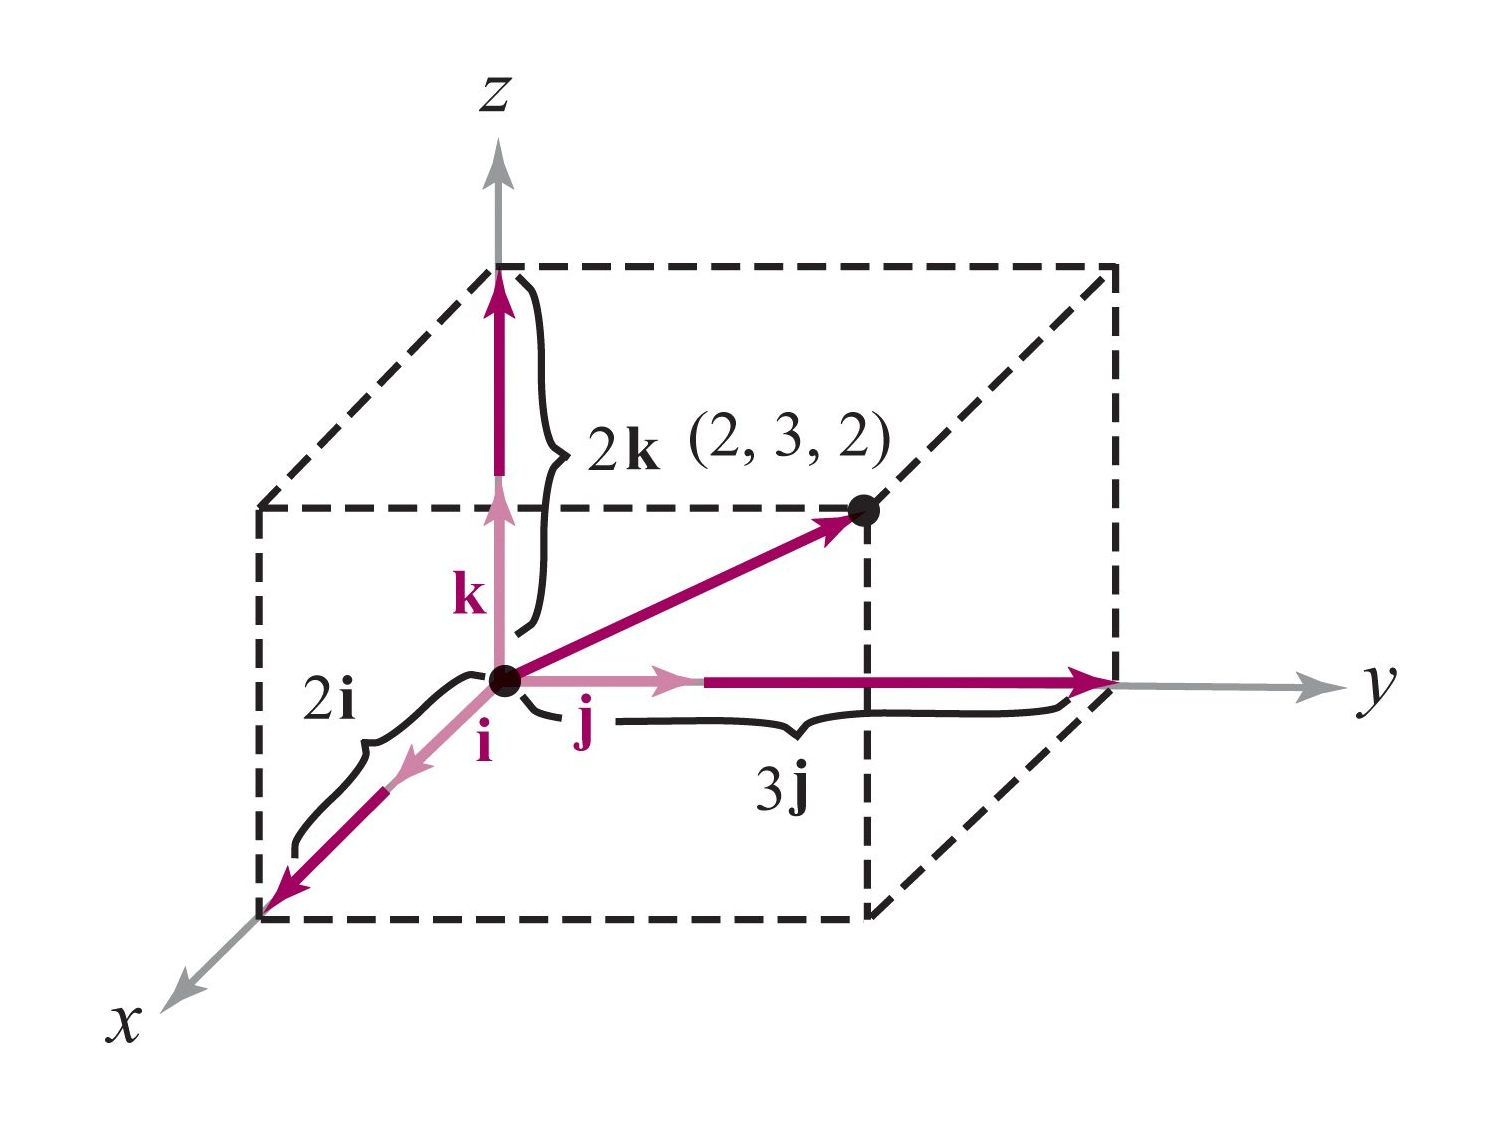
\includegraphics[width=1.15\textwidth]{FIGS/vect_comb_lin_standard_basis_vectors}
		\end{center}
	\end{minipage}
	\vfill
	For $V$ ($\IR^n$), the standard basis vectors are usually denoted $\be_1,\ldots,\be_n$, with 
	\[
	\be_k=(\underbrace{0,\ldots,0}_{k-1},1,\underbrace{0,\ldots,0}_{n-k+1})
	\]
\end{frame}

\begin{frame}
\frametitle{Dot product}
	\begin{definition}[Dot product]
		Let $\ba=(a_1,\ldots,a_n)\in \IR^n$, $\bb=(b_1,\ldots,b_n)\in\IR^n$. 
		The \defword{dot product} of $\ba$ and $\bb$ is the \textbf{scalar}
		\[
		\ba\bullet \bb=\sum_{i=1}^n a_ib_i=a_1b_1+\cdots+a_nb_n
		\]
	\end{definition}
\vfill
The dot product is a special case of \defword{inner product}
\end{frame}

\begin{frame}
\frametitle{Properties of the dot product}
	\begin{theorem}
		For $\ba,\bb,\bc\in \IR^n$ and $\alpha\in\IR$,
		\begin{itemize}
			\item $\ba\bullet\ba=\|\ba\|^2$ \hfill (so $\ba\bullet \ba\geq 0$, with $\ba\bullet \ba=0$ iff $\ba=\b0$)
			\item $\ba\bullet \bb=\bb\bullet \ba$ \hfill ($\bullet$ is commutative)
			\item $\ba\bullet(\bb+\bc)=\ba\bullet \bb+\ba\bullet \bc$ \hfill ($\bullet$ distributive over $+$)
			\item $(\alpha \ba)\bullet \bb=\alpha(\ba\bullet \bb)=\ba\bullet(\alpha \bb)$
			\item $\b0\bullet \ba=0$
		\end{itemize}
	\end{theorem}
\end{frame}

\begin{frame}
\frametitle{Some results stemming from the dot product}
	\begin{theorem}
		If $\theta$ is the angle between the vectors $\ba$ and $\bb$, then
		\[
		\ba\bullet \bb=\|\ba\|\;\|\bb\|\;\cos\theta
		\]
	\end{theorem}
	\begin{corollary}[Cauchy-Schwarz inequality]
		For any two vectors $\ba$ and $\bb$, we have
		\[
		|\ba\bullet \bb|\leq \|\ba\|\;\|\bb\|
		\]
		with equality if and only if $\ba$ is a scalar multiple of $\bb$, or one of them is $\b0$.
	\end{corollary}
	\begin{theorem}
		$\ba$ and $\bb$ are orthogonal if and only if $\ba\bullet \bb=0$.
	\end{theorem}
\end{frame}

\begin{frame}
\frametitle{Scalar and vector projections}
	Scalar projection of $\bv$ onto $\ba$ (or component of $\bv$ along $\ba$):
	\[
  	\mathsf{comp}_{\ba}\bv=
  	\frac{\ba\bullet\bv}{\|\ba\|}
	\]
	\begin{minipage}{0.59\textwidth}
		Vector (or orthogonal) projection of $\bv$ onto $\ba$:
		\[
		\mathsf{proj}_{\ba}\bv=
		  \left(
		    \frac{\ba\bullet\bv}{\|\ba\|}
		  \right)
		  \frac{\ba}{\|\ba\|}
		  =\frac{\ba\bullet\bv}{\|\ba\|^2}\ba
		\]
	\end{minipage}
	\begin{minipage}{0.39\textwidth}
		\begin{center}
			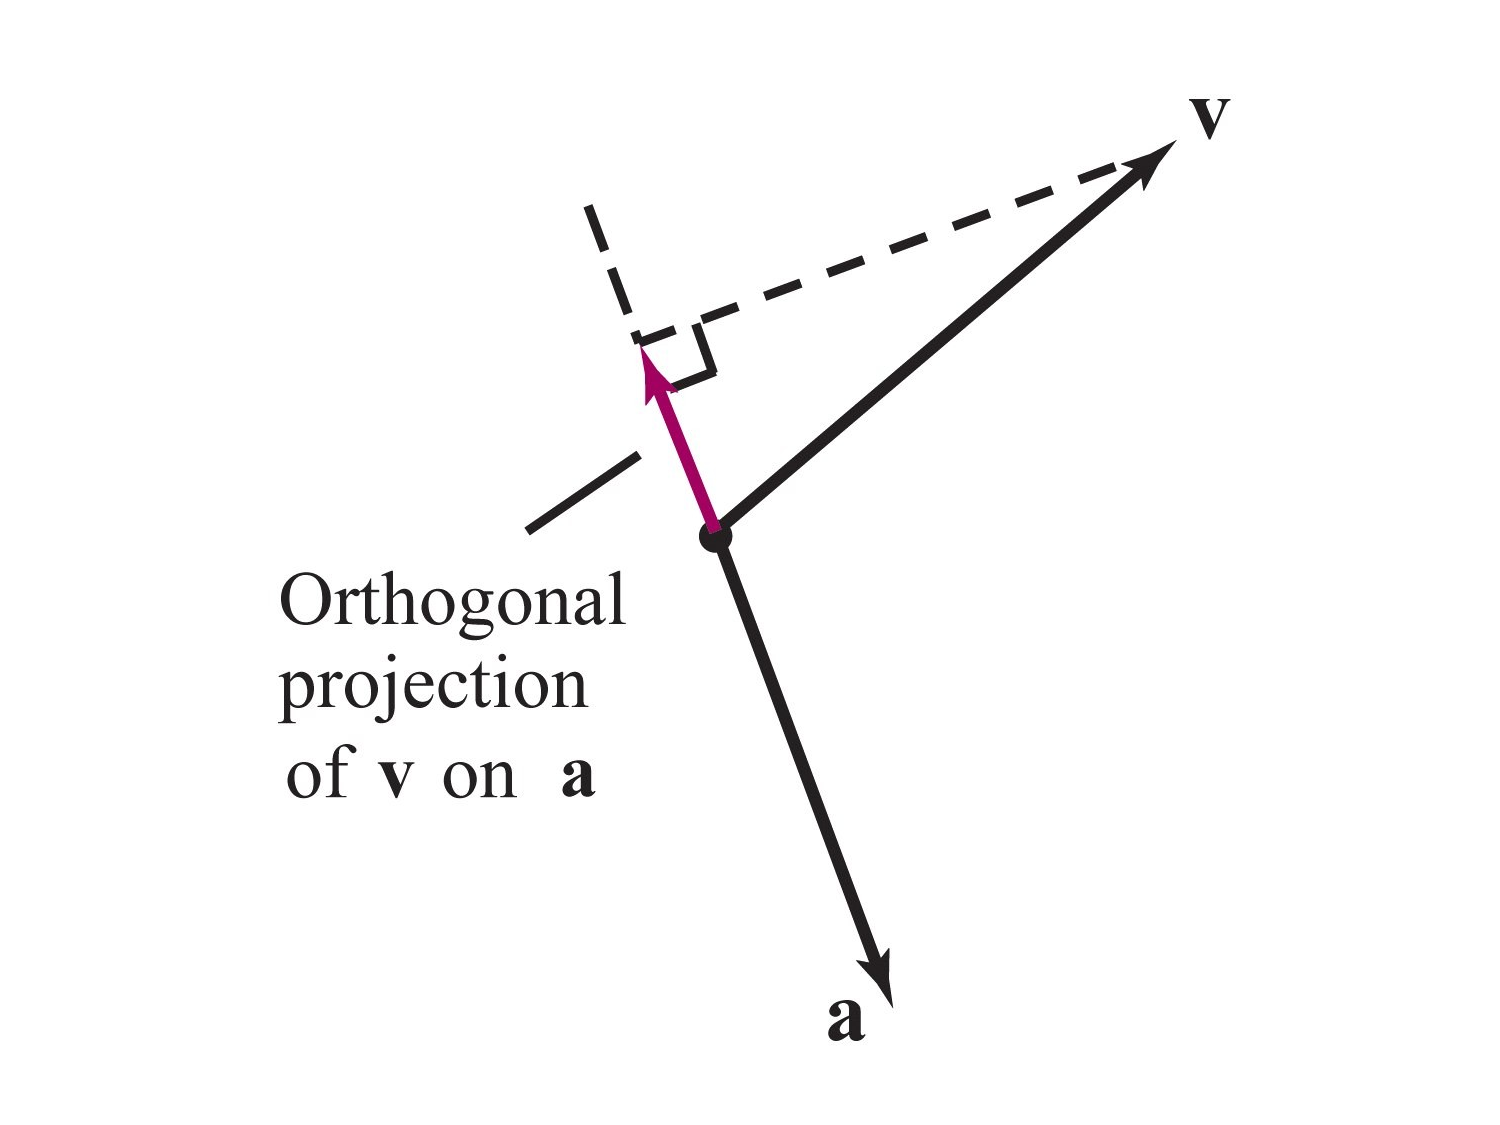
\includegraphics[width=1.1\textwidth]{FIGS/proj_v_onto_a}
		\end{center}
	\end{minipage}
\end{frame}


%%%%%%%%%%%%%%%%%%%%%
%%%%%%%%%%%%%%%%%%%%%
%%%%%%%%%%%%%%%%%%%%%
%%%%%%%%%%%%%%%%%%%%%
\section{Linear systems and matrices}
% The section page
\newSectionSlide{FIGS-slides-admin/a_robot_looking_at_a_desolate_tree_in_the_style_of_Magritte.png}


\begin{frame}{Linear systems}
\begin{definition}[Linear system]
	A \defword{linear system} of $m$ equations in $n$ unknowns takes the form
	\begin{equation}\label{sys:linear_system}
	\begin{matrix}
	a_{11}x_1 &+& a_{12}x_2 &+& \cdots &+& a_{1n}x_n &=& b_1 \\
	a_{21}x_1 &+& a_{22}x_2 &+& \cdots &+& a_{2n}x_n &=& b_2 \\
	\vdots && \vdots && \vdots && \vdots && \vdots \\
	a_{m1}x_1 &+& a_{m2}x_2 &+& \cdots &+& a_{mn}x_n &=& b_n
	\end{matrix}
	\end{equation}
\end{definition}
The $a_{ij}$, $x_j$ and $b_j$ could be in $\IR$ or $\IC$, although here we typically assume they are in $\IR$
\vfill
The aim is to find $x_1,x_2,\ldots,x_n$ that satisfy all equations simultaneously
\end{frame}

\begin{frame}
\begin{importanttheorem}[Nature of solutions to a linear system]
\label{th:nature_solutions_linear_system}
A linear system can have
\begin{itemize}
	\item no solution
	\item a unique solution
	\item infinitely many solutions
\end{itemize}
\end{importanttheorem}
\end{frame}


\begin{frame}{Operations on linear systems}
You learned to manipulate linear systems using
\begin{itemize}
	\item Gaussian elimination
	\item Gauss-Jordan elimination
\end{itemize}
with the aim to put the system in \textbf{row echelon form} (REF) or \textbf{reduced row echelon form} (RREF) 
\end{frame}


\begin{frame}{Matrices and linear systems}
Writing
\[
A=
\begin{pmatrix}
a_{11} & a_{12} & \cdots & a_{1n} \\
a_{21} & a_{22} & \cdots & a_{2n} \\
\vdots &\vdots & & \vdots \\
a_{m1} & a_{m2} & \cdots & a_{mn}
\end{pmatrix},\quad
\bx=
\begin{pmatrix}
x_1\\ x_2 \\ \vdots \\ x_n
\end{pmatrix}
\quad\textrm{and}\quad
\bb=
\begin{pmatrix}
b_1\\ b_2 \\ \vdots \\ b_n
\end{pmatrix}
\]
where $A$ is an $m\times n$ \textbf{matrix}, $\bx$ and $\bb$ are $n$ (column) \textbf{vectors} (or $n\times 1$ matrices), then the linear system in the previous slide takes the form
\[
A\bx=\bb
\]
\end{frame}



\begin{frame}{Notation for vectors}
We usually assume vectors are column vectors and thus write, e.g.,
\[ 
\bx=
\begin{pmatrix}
x_1\\ x_2 \\ \vdots \\ x_n
\end{pmatrix}
= (x_1,x_2,\ldots,x_n)^T
\]
Here, $^T$ is the \textbf{transpose operator} (more on this soon)
\end{frame}



\begin{frame}
Consider the system
\[
A\bx=\bb
\]
\vfill
If $\bb=\b0$, the system is \defword{homogeneous} and always has the solution $\bx=0$ and so the ``no solution'' option in Theorem~\ref{th:nature_solutions_linear_system} goes away
\end{frame}


%%%%%%%%%%%%%%%%%%%%%
%%%%%%%%%%%%%%%%%%%%%
%%%%%%%%%%%%%%%%%%%%%
%%%%%%%%%%%%%%%%%%%%%
\section{Matrix arithmetic}
% The section page
\newSectionSlide{FIGS-slides-admin/a_robot_looking_at_a_desolate_tree_in_the_style_of_Magritte.png}

\begin{frame}
	\begin{definition}[Matrix]
		An $m$-by-$n$ or $m\times n$ matrix is a rectangular array of elements of $\IR$ or $\IC$ with $m$ rows and $n$ columns,
		\[
		A=[a_{ij}]=
		\begin{pmatrix}
		a_{11} & \cdots & a_{1n} \\
		\vdots & & \vdots \\
		a_{m1} & \cdots & a_{mn}
		\end{pmatrix}
		\]
	\end{definition}
	\vfill
	We always list indices as ``row,column''
	\vfill
	We denote $\M_{mn}(\IF)$ or $\IF^{mn}$ the set of $m\times n$ matrices with entries in $\IF=\{\IR,\IC\}$. Often, we omit $\IF$ in $\M_{mn}$ if the nature of $\IF$ is not important
	\vfill
	When $m=n$, we usually write $\M_n$
\end{frame}

\begin{frame}{Basic matrix arithmetic}
Let $A\in\M_{mn},B\in\M_{mn}$ be matrices (of the same size) and $c\in\IF=\{\IR,\IC\}$ be a scalar
\begin{itemize}
	\item \textbf{Scalar multiplication}
	\[
	cA = [ca_{ij}]
	\]
	\item \textbf{Addition}
	\[
	A+B = [a_{ij}+b_{ij}]
	\]
	\item \textbf{Subtraction} (addition of $-B=(-1)B$ to $A$)
	\[
	A-B=A+(-1)B=[a_{ij}+(-1)b_{ij}]=[a_{ij}-b_{ij}]
	\]
	\item \textbf{Transposition} of $A$ gives a matrix $A^T=\M_{nm}$ with
	\[
	A^T=[a_{ji}],\quad j=1,\ldots,n,\quad i=1,\ldots,m
	\]
\end{itemize}
\end{frame}

\begin{frame}{Matrix multiplication}
The (matrix) \textbf{product} of $A$ and $B$, $AB$, requires the ``inner dimensions'' to match, i.e., the number of columns in $A$ must equal the number of rows in $B$
\vfill
Suppose that is the case, i.e., let $A\in\M_{mn}$, $B\in\M_{np}$. Then the $i,j$ entry in $C:=AB$ takes the form
\[
c_{ij} = \sum_{k=1}^n a_{ik}b_{kj}
\]
\vfill
Recall that the matrix product is not commutative, i.e., in general, $AB\neq BA$ (when both those products are defined, i.e., when $A,B\in\M_n$)
\end{frame}

\begin{frame}{Special matrices}
\begin{definition}[Zero and identity matrices]
The \textbf{zero} matrix is the matrix $0_{mn}$ whose entries are all zero.
The \textbf{identity} matrix is a square $n\times n$ matrix $\II_n$ with all entries on the main diagonal equal to one and all off diagonal entries equal to zero
\end{definition}
\begin{definition}[Symmetric matrix]
A square matrix $A\in\M_n$ is \textbf{symmetric} if $\forall i,j=1,\ldots,n$, $a_{ij}=a_{ji}$. In other words, $A\in\M_n$ is symmetric if $A=A^T$
\end{definition}
\end{frame}


\begin{frame}{Properties of symmetric matrices}
\begin{theorem}
\begin{enumerate}
	\item If $A\in\M_n$, then $A+A^T$ is symmetric
	\item If $A\in\M_{mn}$, then $AA^T\in\M_m$ and $A^TA\in\M_n$ are symmetric
\end{enumerate}
\end{theorem}
\vfill
$X$ symmetric $\iff$ $X=X^T$, so use $X=$ the matrix whose symmetric property you want to check

1. True if $A+A^T=(A+A^T)^T$. We have 
\[
(A+A^T)^T=A^T+(A^T)^T=A^T+A=A+A^T
\]

2. $AA^T$ symmetric if $AA^T=(AA^T)^T$. We have 
\[
(AA^T)^T=(A^T)^TA^T=AA^T
\]
$A^TA$ works similarly
\end{frame}

\begin{frame}{Determinants}
\begin{definition}[Determinant]
Let $A\in\M_n$ with $n\geq 2$. The \textbf{determinant} of $A$ is the \emph{scalar}
\[
\det(A)=|A|=\sum_{j=1}^na_{ij}C_{ij}
\]
where $C_{ij}=(-1)^{i+j}\det(A_{ij})$ is the $(i,j)$-\textbf{cofactor} of $A$ and $A_{ij}$ is the submatrix of $A$ from which the $i$th row and $j$th column have been removed
\end{definition}
This is a cofactor expansion along the $i$th row
\vfill
This is a recursive formula: it gives result in terms of $n$ $\M_{n-1}$ matrices, to which it must in turn be applied, all the way down to
\[
\det\left(
\begin{matrix}
a_{11} & a_{12} \\ a_{21} & a_{22}
\end{matrix}\right) = a_{11}a_{22}-a_{12}a_{21}
\]
\end{frame}

\begin{frame}{Two special matrices and their determinants}
\begin{definition}
$A\in\M_n$ is \textbf{upper triangular} if $a_{ij}=0$ when $i>j$, \textbf{lower triangular} if $a_{ij}=0$ when $j>i$, \textbf{triangular} if it is \emph{either} upper or lower triangular and \textbf{diagonal} if it is \emph{both} upper and lower triangular
\end{definition}
When $A$ diagonal, we often write $A=\diag(a_{11},a_{22},\ldots,a_{nn})$
\begin{importanttheorem}
Let $A\in\M_n$ be triangular or diagonal. Then
\[
\det(A)=\prod_{i=1}^n a_{ii}=a_{11}a_{22}\cdots a_{nn}
\]
\end{importanttheorem}
\end{frame}

\begin{frame}{Inversion/Singularity}
\begin{definition}[Matrix inverse]
$A\in\M_n$ is \textbf{invertible} (or \textbf{nonsingular}) if $\exists A^{-1}\in\M_n$ s.t.
\[
AA^{-1}=A^{-1}A=\II
\]
$A^{-1}$ is the \textbf{inverse} of $A$. If $A^{-1}$ does not exist, $A$ is \textbf{singular}
\end{definition}
\begin{importanttheorem}
Let $A\in\M_n$, $\bx,\bb\in\IF^n$. Then
\begin{itemize}
	\item $A$ invertible $\iff$ $\det(A)\neq 0$
	\item If $A$ invertible, $A^{-1}$ is unique
	\item If $A$ invertible, then $A\bx=\bb$ has the unique solution $\bx=A^{-1}\bb$
\end{itemize}
\end{importanttheorem}
\end{frame}

\begin{frame}{Revisiting matrix arithmetic}
With addition, subtraction, scalar multiplication, multiplication, transposition and inversion, you can perform arithmetic on matrices essentially as on scalar, if you bear in mind a few rules
\begin{itemize}
\item The sizes have to be compatible
\item The order is important since matrix multiplication is not commutative
\item Transposition and inversion change the order of products:
\[
(AB)^T=B^TA^T\textrm{ and }(AB)^{-1}=B^{-1}A^{-1}
\]
\end{itemize}
\end{frame}


%%%%%%%%%%%%%%%%%%%%%
%%%%%%%%%%%%%%%%%%%%%
%%%%%%%%%%%%%%%%%%%%%
%%%%%%%%%%%%%%%%%%%%%
\section{Eigenpairs}
% The section page
\newSectionSlide{FIGS-slides-admin/a_robot_looking_at_a_desolate_tree_in_the_style_of_Magritte.png}

\begin{frame}{Eigenvalues / Eigenvectors / Eigenpairs}
\begin{definition}
Let $A\in\M_n$. A vector $\bx\in\IF^n$ such that $\bx\neq\b0$ is an \textbf{eigenvector} of $A$ if $\exists\lambda\in\IF$ called an \textbf{eigenvalue}, s.t.
\[
A\bx=\lambda \bx
\]
A couple $(\lambda,\bx)$ with $\bx\neq\b0$ s.t. $A\bx=\lambda\bx$ is an \textbf{eigenpair}
\end{definition}
If $(\lambda,\bx)$ eigenpair, then for $c\neq 0$, $(\lambda,c\bx)$ also eigenpair since $A(c\bx)=cA\bx=c\lambda\bx$ and dividing both sides by $c$..
\end{frame}




\end{document}
